

%% AAPT Physics Bowl Exams Questions
%%----------------------------------------


%% This section has XX problems


%% PhysicsBowl 2015
%%----------------------------------------
\element{aapt}{ %% Bowl-B4
\begin{question}{bowl-2015-q18}
    A \SI{680}{\hertz} tuning fork is placed over a tube open at both ends that is filled with air.
    As a result, a standing wave in the 3\textsuperscript{rd} harmonic is produced.
    The speed of sound in air is \SI{340}{\meter\per\second}.
    What is the length of the tube?
    \begin{multicols}{3}
    \begin{choices}
        \wrongchoice{\SI{0.38}{\meter}}
        \wrongchoice{\SI{0.67}{\meter}}
      \correctchoice{\SI{0.75}{\meter}}
        \wrongchoice{\SI{1.33}{\meter}}
        \wrongchoice{\SI{1.50}{\meter}}
    \end{choices}
    \end{multicols}
\end{question}
}

\element{aapt}{ %% Bowl-B4
\begin{question}{bowl-2015-q33}
    Two spherical speakers separated by \SI{30.0}{\meter} each emit a
        constant frequency signal of \SI{57.0}{\hertz} in phase with each other.
    The speed of sound in air is \SI{342}{\meter\per\second}.
    \begin{center}
    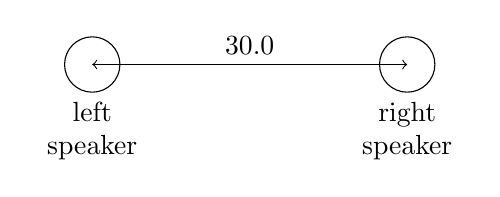
\begin{tikzpicture}
        \draw (-2,0) circle (1em);
        \node[anchor=north,text width=4em,text centered] at (-2,-1em) {left speaker};
        \node[anchor=north,text width=4em,text centered] at (+2,-1em) {right speaker};
        \draw (+2,0) circle (1em);
        \draw[<->] (-2,0) -- (+2,0) node[pos=0.5,anchor=south] {\SI{30.0}{\meter}};
    \end{tikzpicture}
    \end{center}
    How many locations of complete destructive interference of the
        incoming signals are there on the line between the speakers?
    \begin{multicols}{3}
    \begin{choices}
        \wrongchoice{\num{12}}
        \wrongchoice{\num{11}}
      \correctchoice{\num{10}}
        \wrongchoice{\num{9}}
        \wrongchoice{\num{6}}
    \end{choices}
    \end{multicols}
\end{question}
}


%% PhysicsBowl 2014
%%----------------------------------------
\element{aapt}{ %% Bowl-B4
\begin{question}{bowl-2014-q21}
    A tuning fork placed over a \SI{57}{\centi\meter} column of air closed only at its bottom end produces a standing wave in the 3\textsuperscript{rd} harmonic.
    The speed of sound in air is \SI{342}{\meter\per\second}.
    What is the frequency of the tuning fork?
    \begin{multicols}{3}
    \begin{choices}
        \wrongchoice{\SI{150}{\hertz}}
        \wrongchoice{\SI{300}{\hertz}}
      \correctchoice{\SI{450}{\hertz}}
        \wrongchoice{\SI{600}{\hertz}}
        \wrongchoice{\SI{900}{\hertz}}
    \end{choices}
    \end{multicols}
\end{question}
}

\element{aapt}{ %% Bowl-B4
\begin{question}{bowl-2014-q28}
    A standing wave is created in an air-filled tube open at both ends when a tuning fork of frequency \SI{552}{\hertz} is placed near one of the open ends.
    A tuning fork of frequency \SI{644}{\hertz} produces the next highest harmonic for this tube.
    What is the length of the open tube?
    Assume room temperature.
    \begin{choices}
        \wrongchoice{$f_{water}=f_{air}$; $\lambda_{water}=\lambda{air}$; $v_{water}=v_{air}$}
      \correctchoice{$f_{water}=f_{air}$; $\lambda_{water}>\lambda{air}$; $v_{water}>v_{air}$}
        \wrongchoice{$f_{water}<f_{air}$; $\lambda_{water}>\lambda{air}$; $v_{water}=v_{air}$}
        \wrongchoice{$f_{water}<f_{air}$; $\lambda_{water}=\lambda{air}$; $v_{water}<v_{air}$}
        \wrongchoice{$f_{water}=f_{air}$; $\lambda_{water}<\lambda{air}$; $v_{water}>v_{air}$}
    \end{choices}
\end{question}
}


%% PhysicsBowl 2013
%%----------------------------------------
\element{aapt}{ %% Bowl-B4
\begin{question}{bowl-2013-q34}
    Which one of the following choices represents the base MKS units for sound intensity?
    \begin{choices}
      \correctchoice{kilogram per second cubed (\si{\kilo\gram\per\second\cubed})}
        \wrongchoice{meter per kilogram per second dubed (\si{\meter\per\kilo\gram\per\second\cubed})}
        \wrongchoice{meter squared per kilogram per second squared (\si{\meter\squared\per\kilo\gram\per\second\squared})}
        \wrongchoice{kilogram per meter per second squared (\si{\kilo\gram\per\meter\per\second\squared})}
        \wrongchoice{second squared per meter per kilogram (\si{\second\squared\per\meter\per\kilo\gram})}
    \end{choices}
\end{question}
}


%% PhysicsBowl 2011
%%----------------------------------------
\element{aapt}{ %% Bowl-B4
\begin{question}{bowl-2011-q43}
    A standing wave is created in an air-filled tube open
        at both ends when a tuning fork of frequency
        \SI{552}{\hertz} is placed near one of the open ends.
    A tuning fork of frequency \SI{644}{\hertz} produces
        the next highest harmonic for this tube.
    What is the length of the open tube?
    Assume room temperature.
    \begin{multicols}{3}
    \begin{choices}
        \wrongchoice{\SI{0.46}{\meter}}
        \wrongchoice{\SI{0.92}{\meter}}
        \wrongchoice{\SI{1.59}{\meter}}
      \correctchoice{\SI{1.85}{\meter}}
        \wrongchoice{\SI{3.70}{\meter}}
    \end{choices}
    \end{multicols}
\end{question}
}


%% PhysicsBowl 2010
%%----------------------------------------
\element{aapt}{ %% Bowl-B4
\begin{question}{bowl-2010-q17}
    A tube of air open at only one end is vibrating in
        the 5\textsuperscript{th} harmonic from a tuning
        fork of frequency \SI{120}{\hertz} placed at the open end.
    If the tube of air were to vibrate at its fundamental
        frequency, what frequency tuning fork would be needed at the open end?
    \begin{multicols}{3}
    \begin{choices}
      \correctchoice{\SI{24}{\hertz}}
        \wrongchoice{\SI{30}{\hertz}}
        \wrongchoice{\SI{40}{\hertz}}
        \wrongchoice{\SI{125}{\hertz}}
        \wrongchoice{\SI{600}{\hertz}}
    \end{choices}
    \end{multicols}
\end{question}
}


%% PhysicsBowl 2008
%%----------------------------------------
\element{aapt}{ %% Bowl-B4
\begin{question}{bowl-2008-q18}
    A car is moving to the left at \SI{20}{\meter\per\second} while a truck is moving to the right at \SI{25}{\meter\per\second}.
    If the truck emits a sound of frequency \SI{5000}{\hertz},
        what is the perceived frequency of the sound by the driver of the car?
    Assume the vehicles are moving directly away from each other on a \SI{20.0}{\degreeCelsius} day.
    \begin{multicols}{3}
    \begin{choices}
      \correctchoice{\SI{4384}{\hertz}}
        \wrongchoice{\SI{4706}{\hertz}}
        \wrongchoice{\SI{4932}{\hertz}}
        \wrongchoice{\SI{5079}{\hertz}}
        \wrongchoice{\SI{5714}{\hertz}}
    \end{choices}
    \end{multicols}
\end{question}
}

\element{aapt}{ %% Bowl-B4
\begin{question}{bowl-2008-q27}
    A tube of length $L_1$ is open at both ends.
    A second tube of length $L_2$ is closed at one end and open at the other end.
    This second tube resonates at the same fundamental frequency as the first tube.
    What is the value of $L_2$?
    \begin{multicols}{3}
    \begin{choices}
        \wrongchoice{$4L_1$}
        \wrongchoice{$2L_1$}
        \wrongchoice{$L_1$}
        \wrongchoice{$\dfrac{1}{2}L_1$}
        \wrongchoice{$\dfrac{1}{4}L_1$}
    \end{choices}
    \end{multicols}
\end{question}
}


%% PhysicsBowl 2006
%%----------------------------------------
\element{aapt}{ %% Bowl-B4
\begin{question}{bowl-2006-q31}
    A sound increases its decibel reading from \SIrange{20}{40}{\decibel}.
    This means that the intensity of the sound:
    \begin{choices}
        \wrongchoice{is doubled}
        \wrongchoice{is 20 times greater}
      \correctchoice{is 100 times greater}
        \wrongchoice{is the old intensity + 20}
        \wrongchoice{is the old intensity + 100}
    \end{choices}
\end{question}
}


%% PhysicsBowl 2005
%%----------------------------------------
\element{aapt}{ %% Bowl-B4
\begin{question}{bowl-2005-q09}
    A tube is open at both ends with the air oscillating in the $4^{th}$ harmonic.
    How many displacement nodes are located within the tube?
    \begin{multicols}{3}
    \begin{choices}
        \wrongchoice{\num{2}}
        \wrongchoice{\num{3}}
      \correctchoice{\num{4}}
        \wrongchoice{\num{5}}
        \wrongchoice{\num{6}}
    \end{choices}
    \end{multicols}
\end{question}
}

\element{aapt}{ %% Bowl-B4
\begin{question}{bowl-2005-q23}
    A person hears a single-frequency sound from a speaker that emits sound uniformly in all directions.
    The person records the decibel level reading.
    Which of the following processes would increase the decibel reading the most?
    \begin{choices}
        \wrongchoice{The power output of the speaker is doubled.}
      \correctchoice{The distance of the person to the speaker is halved.}
        \wrongchoice{The frequency of the sound is doubled.}
        \wrongchoice{The temperature of the air is doubled on the Kelvin scale.}
        \wrongchoice{The area over which the sound is transmitted is halved.}
    \end{choices}
\end{question}
}

\element{aapt}{ %% Bowl-B4
\begin{question}{bowl-2005-q47}
    A sound wave generated from a tuning fork of single frequency travels from air (with speed of sound \SI{340}{\meter\per\second}) into rock (with speed of sound \SI{1500}{\meter\per\second}).
    Which statement is true about the wavelength and frequency of the sound as it passes from air to rock?
    \begin{choices}
        \wrongchoice{The frequency of the sound increases and the wavelength increases.}
        \wrongchoice{The frequency of the sound increases and the wavelength is unchanged.}
        \wrongchoice{The frequency of the sound is unchanged and the wavelength is decreased.}
      \correctchoice{The frequency of the sound is unchanged and the wavelength is increased.}
        \wrongchoice{The frequency of the sound decreases and the wavelength increased.}
    \end{choices}
\end{question}
}


%% PhysicsBowl 2000
%%----------------------------------------
\element{aapt}{ %% Bowl-B4
\begin{question}{bowl-2000-q33}
    %The next TWO questions refer to the following information.
    A natural horn (trumpet with no valves) is similar to an pipe open at both ends.
    A musician plans to create a fundamental frequency of
        \SI{256}{\hertz} (middle $C$) using the horn.
    %% start question
    If sound travels at \SI{350}{\meter\per\second},
        what must be the length of this horn?
    \begin{multicols}{2}
    \begin{choices}
        \wrongchoice{\SI{0.34}{\meter}}
      \correctchoice{\SI{0.68}{\meter}}
        \wrongchoice{\SI{0.73}{\meter}}
        \wrongchoice{\SI{1.36}{\meter}}
        \wrongchoice{\SI{1.46}{\meter}}
    \end{choices}
    \end{multicols}
\end{question}
}

\element{aapt}{ %% Bowl-B4
\begin{question}{bowl-2000-q34}
    %The next TWO questions refer to the following information.
    A natural horn (trumpet with no valves) is similar to an pipe open at both ends.
    A musician plans to create a fundamental frequency of
        \SI{256}{\hertz} (middle $C$) using the horn.
    %% start question
    A talented musician can produce a number of overtones on this natural horn.
    What would be the frequency of the fourth overtone produced when the
        musician is playing a middle $C$ fundamental?
    \begin{multicols}{2}
    \begin{choices}
        \wrongchoice{\SI{512}{\hertz}}
        \wrongchoice{\SI{768}{\hertz}}
        \wrongchoice{\SI{1024}{\hertz}}
      \correctchoice{\SI{1280}{\hertz}}
        \wrongchoice{\SI{1536}{\hertz}}
    \end{choices}
    \end{multicols}
\end{question}
}


%% PhysicsBowl 1998
%%----------------------------------------
\element{aapt}{ %% Bowl-B4
\begin{question}{bowl-1998-q18}
    When a train is at rest,
        both a passenger on the train and a ticket seller on the station agree that the trains whistle produces sound at a frequency of \SI{120}{\hertz}.
    When the train is moving away from the station at \SI{15}{\meter\per\second},
        the passenger hears a frequency of \rule[-0.1pt]{4em}{0.1pt} and the ticket seller hears a frequency of \rule[-0.1pt]{4em}{0.1pt}.
    \begin{multicols}{2}
    \begin{choices}
        \wrongchoice{\SI{120}{\hertz}, \SI{125}{\hertz}}
        \wrongchoice{\SI{115}{\hertz}, \SI{120}{\hertz}}
        \wrongchoice{\SI{120}{\hertz}, \SI{120}{\hertz}}
        \wrongchoice{\SI{115}{\hertz}, \SI{115}{\hertz}}
      \correctchoice{\SI{120}{\hertz}, \SI{115}{\hertz}}
    \end{choices}
    \end{multicols}
\end{question}
}

\element{aapt}{ %% Bowl-B4
\begin{question}{bowl-1998-q35}
    A pipe that is closed at one end and open at the other resonates at a fundamental frequency of \SI{240}{\hertz}.
    The next lowest/highest frequency it resonates at is most nearly:
    \begin{multicols}{3}
    \begin{choices}
        \wrongchoice{\SI{60}{\hertz}}
        \wrongchoice{\SI{80}{\hertz}}
        \wrongchoice{\SI{120}{\hertz}}
        \wrongchoice{\SI{480}{\hertz}}
      \correctchoice{\SI{720}{\hertz}}
    \end{choices}
    \end{multicols}
\end{question}
}


%% PhysicsBowl 1996
%%----------------------------------------
\element{aapt}{ %% Bowl-B4
\begin{question}{bowl-1996-q03}
    If the frequency of sound is doubled, the wavelength:
    \begin{choices}
      \correctchoice{halves and the speed remains unchanged.}
        \wrongchoice{doubles and the speed remains unchanged.}
        \wrongchoice{is unchanged and the speed doubles.}
        \wrongchoice{is unchanged and the speed halves.}
        \wrongchoice{the wavelength halves and the speed halves.}
    \end{choices}
\end{question}
}


%% PhysicsBowl 1995
%%----------------------------------------
\element{aapt}{ %% Bowl-B4
\begin{question}{bowl-1995-q01}
    Which is not associated with a sound wave?
    \begin{multicols}{2}
    \begin{choices}
        \wrongchoice{amplitude}
        \wrongchoice{period}
      \correctchoice{polarization}
        \wrongchoice{velocity}
        \wrongchoice{wavelength}
    \end{choices}
    \end{multicols}
\end{question}
}


\endinput


